\documentclass[../main.tex]{subfiles}
\graphicspath{{\subfix{../imgs/}}}
\begin{document}

\chapter{Material y Método} \label{cap:met}
Durante este capítulo se explican las diferentes herramientas concretas que han servido de ingredientes en la realización de este trabajo. A la hora desgranar los diferentes agentes que entran en acción, se realiza previamente una clasificación entre software y hardware que se refleja en las secciones de este capítulo.

\section{Hardware}  \label{section:met-hardware}
Dentro del material hardware dispuesto se distinguen aeronaves, dispositivos embebidos y sensores de visión. Dichos elementos se abordarán en los próximos apartados.

\subsection{Aeronaves} \label{section:met-aeronaves}
En coherencia con los objetivos del proyecto, se han seleccionado tres diferentes aeronaves sobre las que realizar las pruebas del software desarrollado. La elección de estas aeronaves se ha realizado con el propósito de cubrir un amplio abanico de opciones, siendo los tres cuadri-cópteros muy diferentes entre ellos. Entre las seleccionadas se encuentran aeronaves reales y simuladas, aeronaves propietarias y libres, y aeronaves de vuelo en interiores o en exteriores. Cubrir una gran variedad de posibilidades supone dotar al software de una alta versatilidad, siendo en un futuro más fácilmente extensible a otras plataformas.

Las aeronaves elegidas son:
\begin{enumerate}
    \item \textbf{3DR Iris simulado.}
    \item \textbf{DJI Tello.}
    \item \textbf{PX4 de construcción propia.}
\end{enumerate}

En primer lugar se encuentra una aeronave simulada, 3DR Iris de 3D Robotics. Utilizar una aeronave simulada en las primeras fases del desarrollo supone grandes ventajas en ahorro de tiempo y coste, pues los errores en el código no suponen un daño en el material. \\
La aeronave utiliza PX4 como autopiloto y se simula mediante Gazebo. Se darán más detalles acerca de esta aeronave en la sección de software (Sec. \ref{section:met-sim}).

La segunda aeronave seleccionada es el DJI Tello (Fig. \ref{fig:tello}). Es una aeronave propietaria (del fabricante chino \emph{DJI}) pensada para vuelos en interiores debido a su pequeño tamaño y peso (ver Tabla \ref{tab:tello}). Incluye un sensor telemétrico (\emph{optical flow}) y un barómetro, para cálculos de odometría, un sensor de visión y una antena WiFi para las comunicaciones. 

\begin{table}[H]
	\ttabbox[\FBwidth]
	{\caption{Especificaciones del DJI Tello.} \label{tab:tello}}
	{\begin{tabular}{|c|c|}
		\hline
		\textbf{Características} & \textbf{Valores} \\
		\hline
		Peso (g)             & 80 \\
		\hline
        Tamaño (mm)          & 98×92.5×41 \\
        \hline
        Distancia máx. (m)   & 100 \\
        \hline
        Velocidad máx. (m/s) & 10 \\
        \hline
        Tiempo máx. (min)    & 13 \\
        \hline
        Altura máx. (m)      & 30 \\
        \hline
        Cámara (MP)          & 5 \\
        \hline
        FOV (º)              & 82.6 \\
        \hline
        Vídeo                & HD 720p 30 fps \\
        \hline
		\multicolumn{2}{l}{Fuente: DJI}
	\end{tabular}}
\end{table}

Debido a sus características es ideal para realizar los primeros ensayos de navegación en interiores. Su tamaño y peso aseguran daños limitados a terceros en caso de accidente, y pese a su apariencia es una aeronave robusta y con grandes prestaciones de vuelo. Además, el propio fabricante ofrecen un kit de desarrollo (SDK) para la programación de aplicaciones sobre el dron. \\
Sin embargo, su uso es limitado por la comunicación con la estación terrestre, debido a que el procesamiento no se puede realizar a bordo de la aeronave.  

\begin{figure}[!ht]
 	\ffigbox[\FBwidth] {
 	    \caption[DJI Tello]{DJI Tello.}
        \label{fig:tello}
 	}
 	{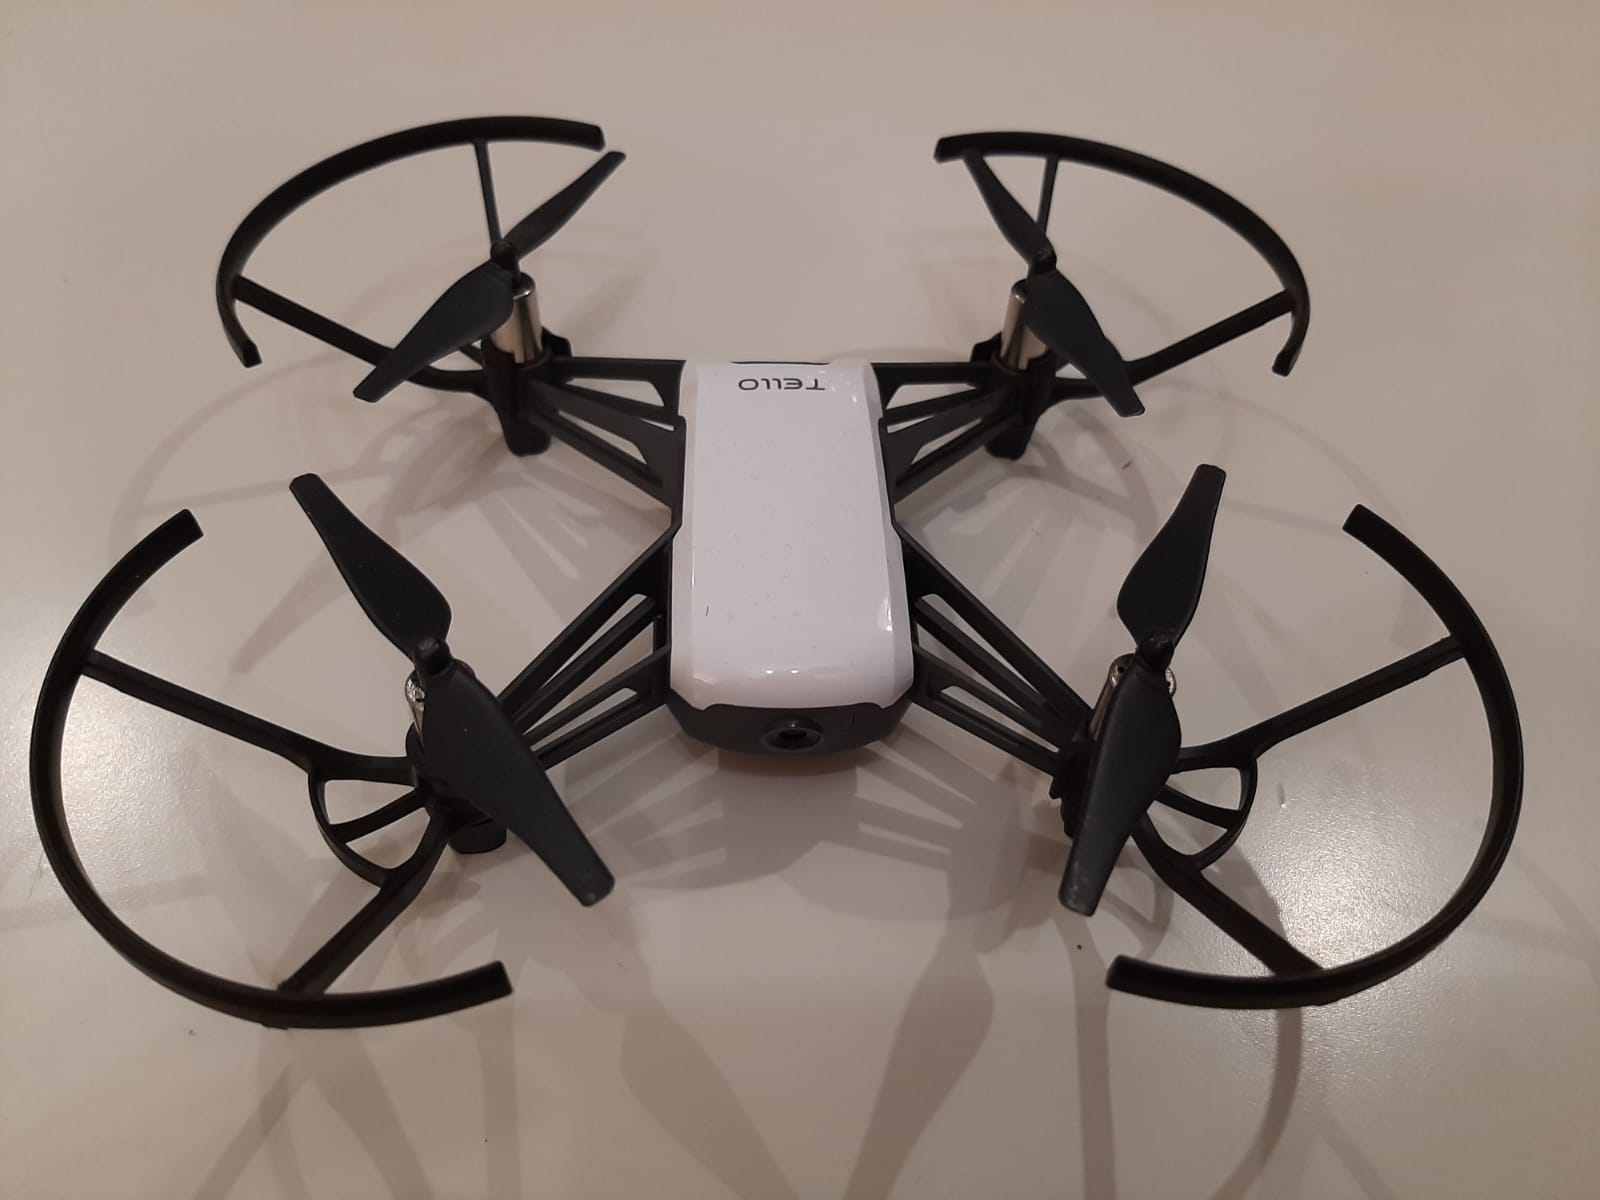
\includegraphics[width=0.7\textwidth]{03/tello.jpg}}
\end{figure}

En tercer lugar, se ha elegido un dron de construcción propia y desarrollado por A. Madridano en su tesis doctoral \cite{madridano2020arquitectura} junto al Laboratorio de Sistemas Inteligentes (LSI) de la Universidad Carlos III de Madrid (UC3M) \cite{lsi}. La aeronave posee una controladora PixHawk v1, con el autopiloto PX4 en su última versión estable (v1.12.3). La aeronave lleva a bordo un ordenador de cómputo que permite realizar el procesamiento de la información in-situ. Además incluye una antena GPS, un receptor de telemetría y una antena WiFi, entre otros sensores. La Tabla \ref{tab:px4} recoge las características principales de la aeronave.

\begin{table}[H]
	\ttabbox[\FBwidth]
	{\caption{Especificaciones del dron de construcción propia.} \label{tab:px4}}
	{\begin{tabular}{|c|c|}
		\hline
		\textbf{Características} & \textbf{Valores} \\
		\hline
		Peso (Kg)             & 2,5 \\  % tesis angel
		\hline
        Tamaño (mm)          & 340×340x250 \\  % tesis angel
        \hline
        Distancia máx. (m)   & 1000 \\  % vision directa (legislacion)
        \hline
        Velocidad máx. (m/s) & 12 \\  % px4 default horizontal cruise speed
        %\hline
        %Tiempo máx. (min)    & ? \\
        \hline
        Altura máx. (m)      & 120 \\ % legislacion
        \hline
		\multicolumn{2}{l}{Fuente: Elaboración propia \cite{madridano2020arquitectura}.}
	\end{tabular}}
\end{table}

Dicha aeronave está pensada para su uso en las últimas fases del desarrollo al ser la aeronave más potente de las tres. Al realizar a bordo el procesamiento, permite realizar tareas más complejas en exteriores sin limitaciones con la comunicación con la estación terrestre, ya que esta es prescindible. La Figura \ref{fig:px4-real} muestra el cuadri-cóptero.

\begin{figure}[!ht]
 	\ffigbox[\FBwidth] {
 	    \caption[Dron no comercial]{Dron no comercial.}
        \label{fig:px4-real}
    }
 	{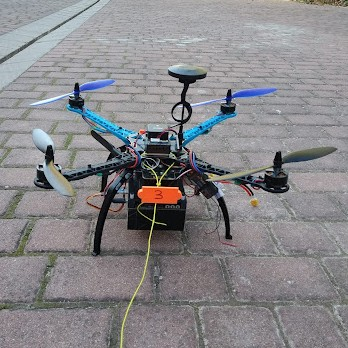
\includegraphics[width=0.75\textwidth]{03/px4-real2.jpg}}
\end{figure}

\subsection{Dispositivos embebidos} \label{section:met-embeb}
En la apartado anterior, con la última aeronave se ha presentado un dispositivo embebido. Estos equipos están presentes cuando existe interés de embarcar parte del software en la aeronave. Ejecutar ciertos procesos en la aeronave ofrece un salto de rendimiento en algoritmos en tiempo real, muy presentes en la visión por computador. Además, al tratarse de vehículos aéreos no es posible en muchos casos ejecutar estos algoritmos en ordenadores portátiles como sí se hace tradicionalmente en vehículos terrestres, debido a la latencia en las comunicaciones. Una alta latencia dificulta cerrar el ciclo de control en el segmento tierra, que se ve limitada por la distancia a la estación de tierra.

Por ello, debido al mencionado aumento de interés en aplicaciones de visión en tiempo real ha propiciado el desarrollo de dispositivos embebidos de baja potencia para su integración en sistemas robóticos móviles. Ejemplo de ello son los dispositivos como Arduino \cite{arduino} o Raspberry Pi \cite{raspberry}, utilizados en pequeños robots como PiBot \cite{vega2018pibot} (ver Fig. \ref{fig:pibot}) o el GoPiGo \cite{gopigo}.

\begin{figure}[!ht]
 	\ffigbox[\FBwidth] {
 	    \caption[PiBot]{PiBot.}
        \label{fig:pibot}
    }
 	{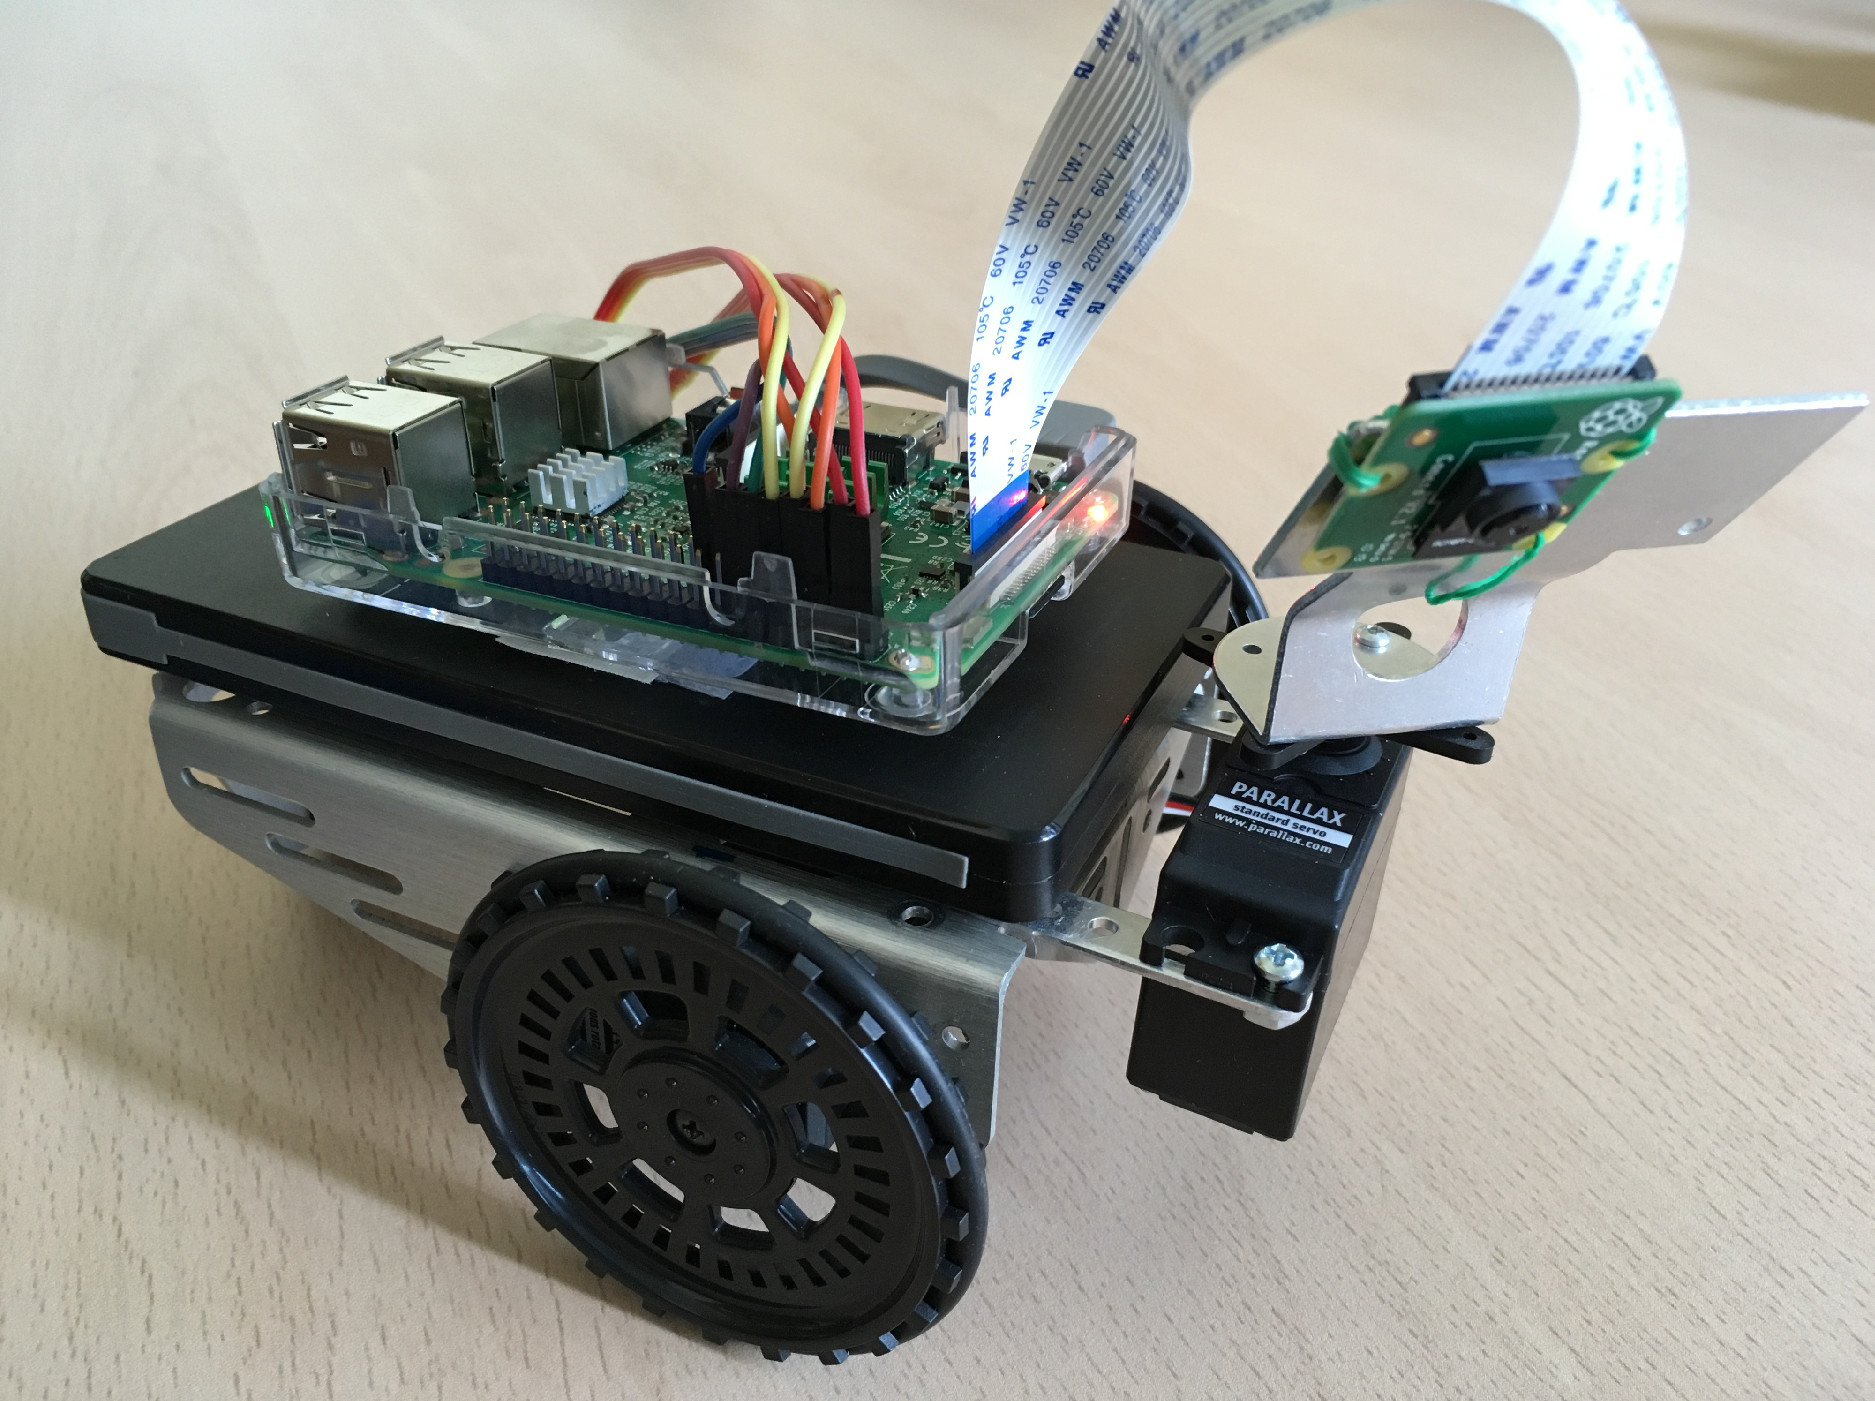
\includegraphics[width=0.6\textwidth]{03/pibot.jpg}}
\end{figure}

Sin embargo, para ejecutar algoritmos complejos, como redes neuronales, no es suficiente con los dispositivos mencionados y es necesario utilizar dispositivos específicos. Una alternativa viable son los dispositivos \emph{Jetson} fabricados por \emph{NVIDIA} \cite{jetson}. Cada NVIDIA Jetson es un sistema en módulo (SOM) completo que incluye CPU, GPU, memoria, administración de energía, interfaces de alta velocidad y más, que permiten ejecutar CUDA \cite{cuda}, una biblioteca de computación paralela de bajo nivel, así como varios kits de herramientas (como JetPack SDK \cite{jetpack}) diseñados para optimizar los procesos que se ejecuten en el dispositivo. \\
El tamaño y consumo de estos dispositivos hacen que sea sistemas ideales para embarcar en vehículos aéreos. Existen diferentes modelos disponibles como la Jetson Nano, la Jetson TX2 o la Jetson AGX Xavier, seleccionada para embarcar en la aeronave. La Figura \ref{fig:xavier} muestra los principales elementos del dispositivo, mientras que la Tabla \ref{tab:xavier} recoge sus características.

\begin{table}[H]
	\ttabbox[\FBwidth]
	{\caption{Especificaciones de Jetson AGX Xavier.} \label{tab:xavier}}
	{\begin{tabular}{|c|c|}
		\hline
		\textbf{Características} & \textbf{Valores} \\
		\hline
		Peso (g)        & 630 \\
		\hline
        Tamaño (mm)     & 100×86 \\
        \hline
        Potencia (W)    & 10 | 15 | 30 \\
        \hline
        GPU             & Volta  64 Tensor Cores \\
        \hline
        CPU             & 8-Core ARM 64-Bit \\
        \hline
        Rendimiento (TFLOPS) & 11 \\
        \hline
        Memoria (GB)    & 16 \\
        \hline 
        Almacenamiento (GB)    & 32 \\
        \hline
		\multicolumn{2}{l}{Fuente: NVIDIA}
	\end{tabular}}
\end{table}

\begin{figure}[!ht]
 	\ffigbox[\FBwidth] {
 	    \caption[NVIDIA Jetson AGX Xavier]{NVIDIA Jetson AGX Xavier.}
        \label{fig:xavier}
    }
 	{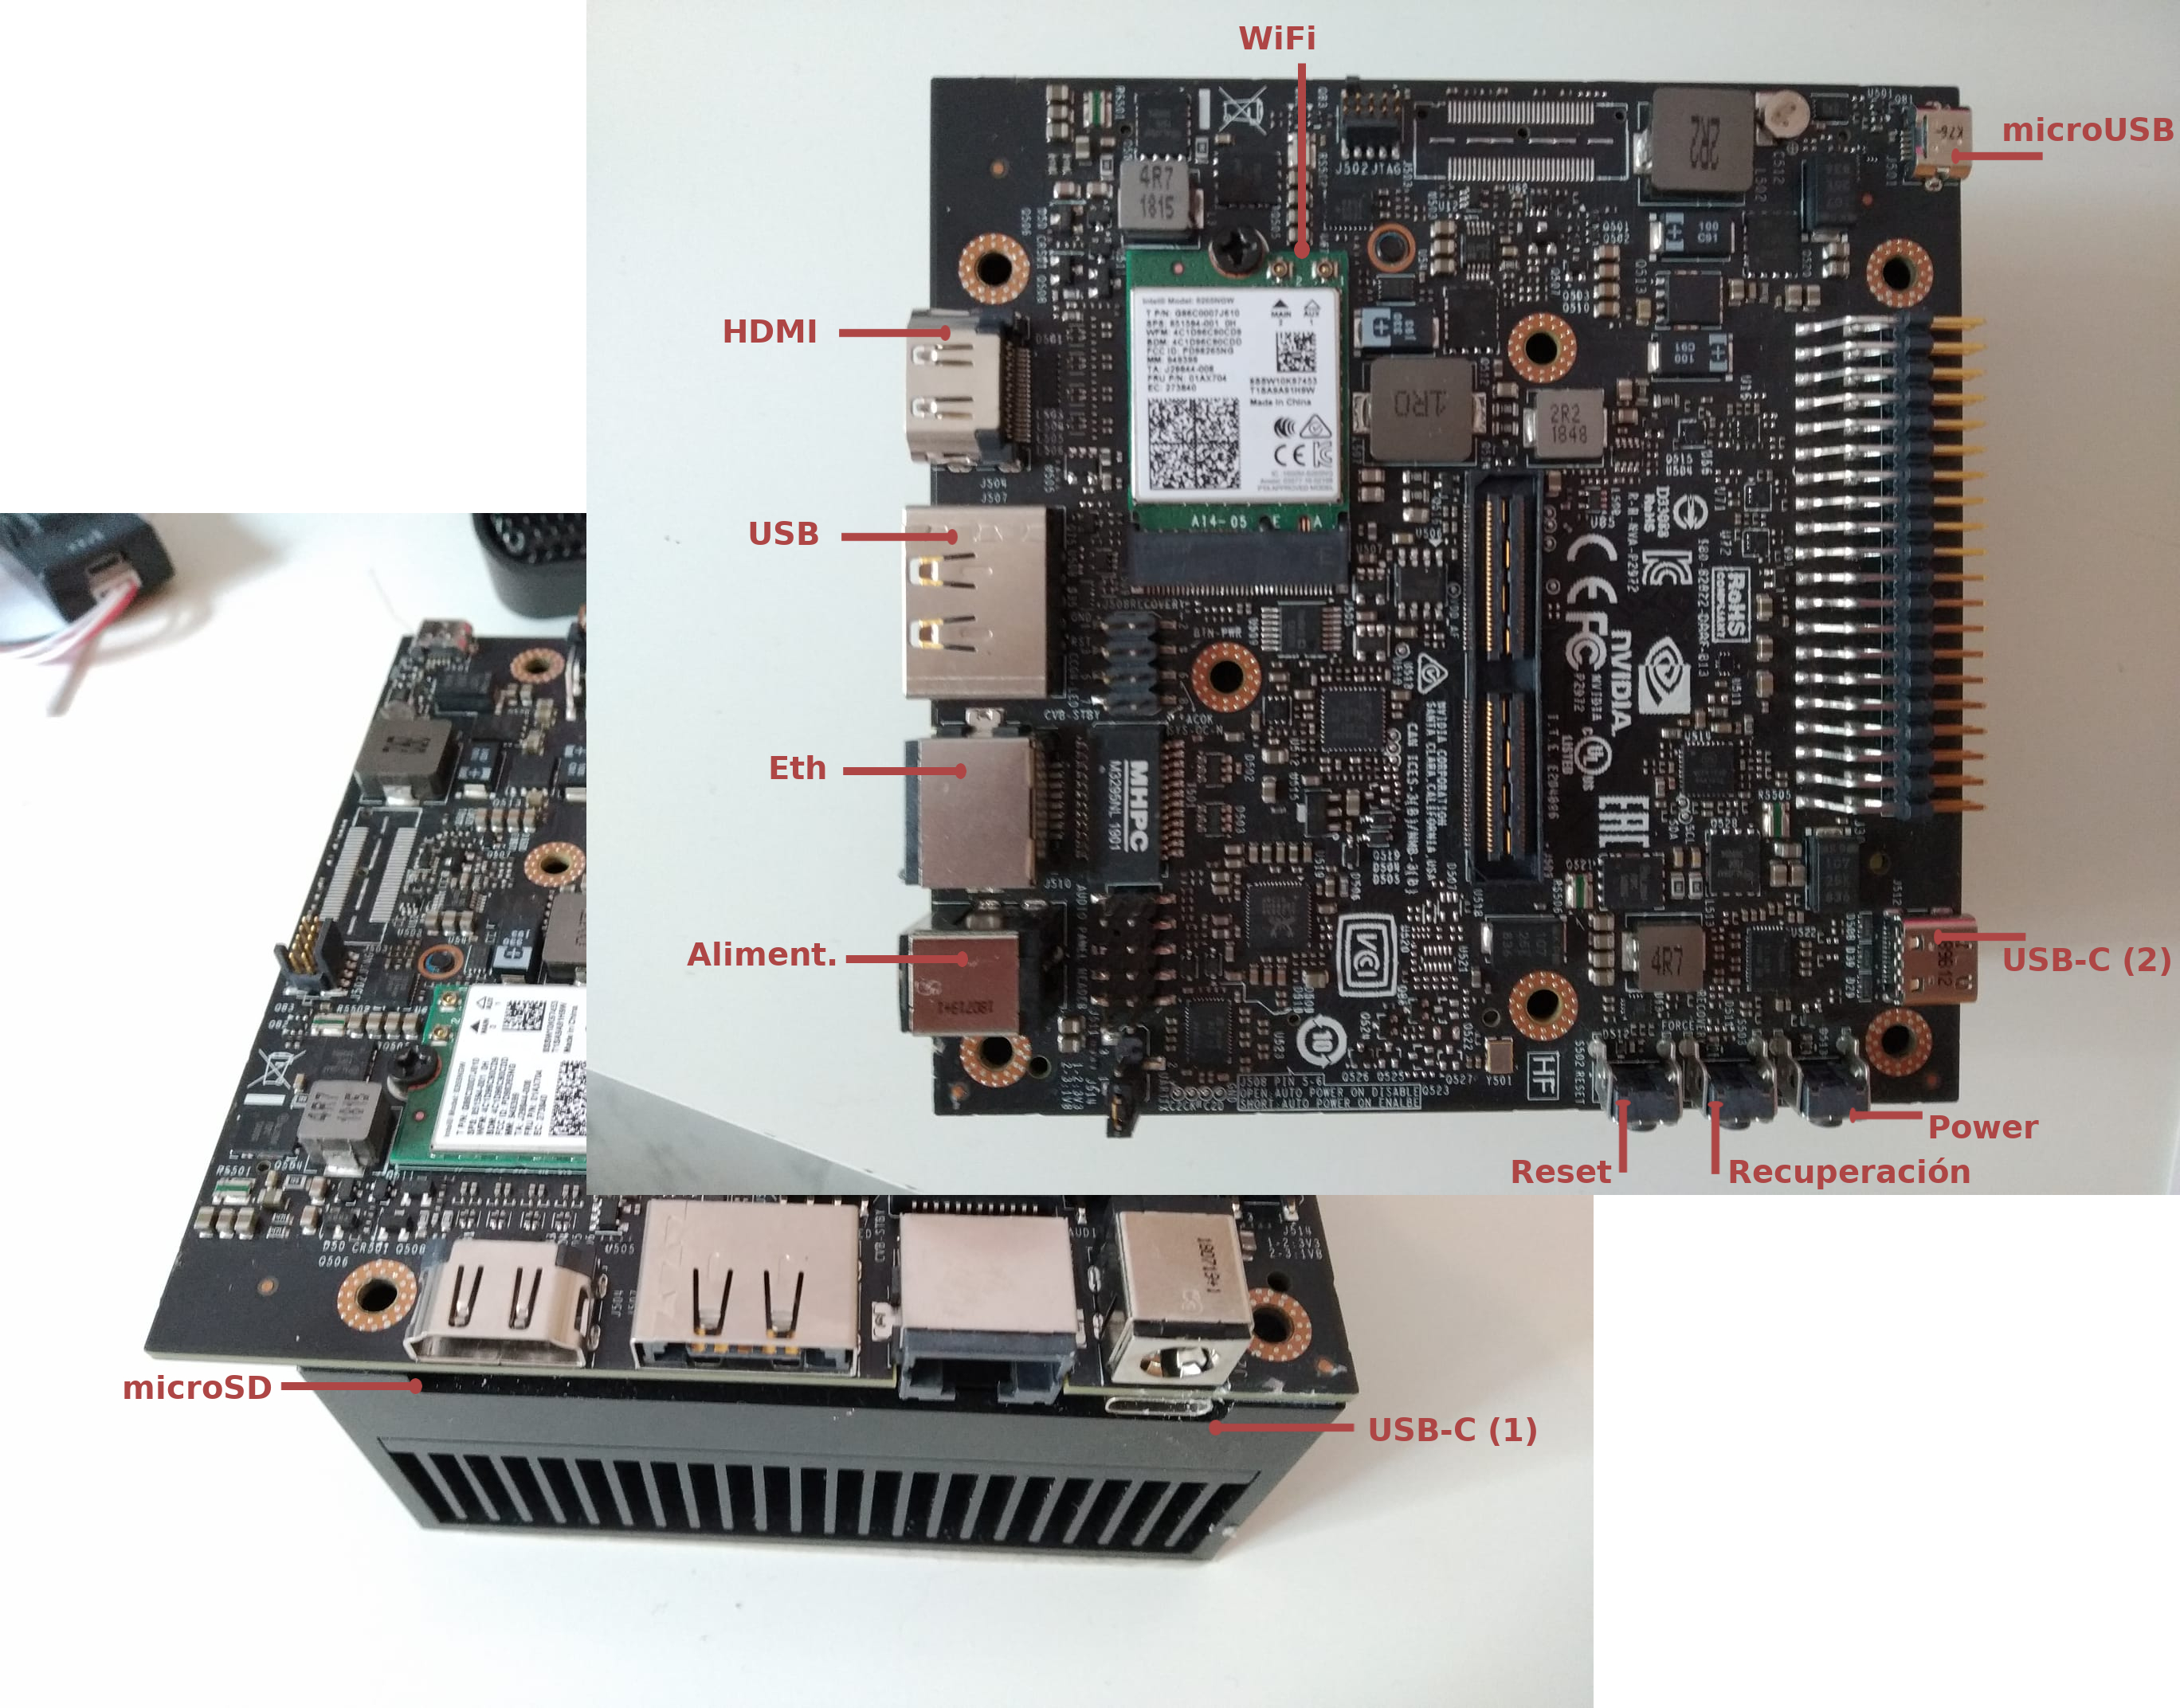
\includegraphics[width=\textwidth]{03/xavier-descrip.jpg}}
\end{figure}

\clearpage
\subsection{Sensores de visión} \label{section:met-visión}
Para el desarrollo de aplicaciones de control visual, es necesario poseer un sensor de visión a bordo de la aeronave. Tanto la aeronave simulada como el Tello poseen una cámara embarcada, en el primer caso un sensor simulado (del cual se darán más detalles en la Sec. \ref{section:met-sim}), mientras que en el segundo el sensor viene integrado en el propio dron. \\
Sin embargo, para el dron de desarrollo propio es necesario seleccionar una cámara, ya que el diseño inicial no incluye ninguna. A la hora de elegir el sensor, se ha apostado por el uso de un sensor RGB básico, teniendo un sistema similar al de resto de las aeronaves.

\begin{figure}[!ht]
 	\ffigbox[\FBwidth] {
 	    \caption[Cámara Victure AC600]{Cámara Victure AC600.}
        \label{fig:victure}
    }
 	{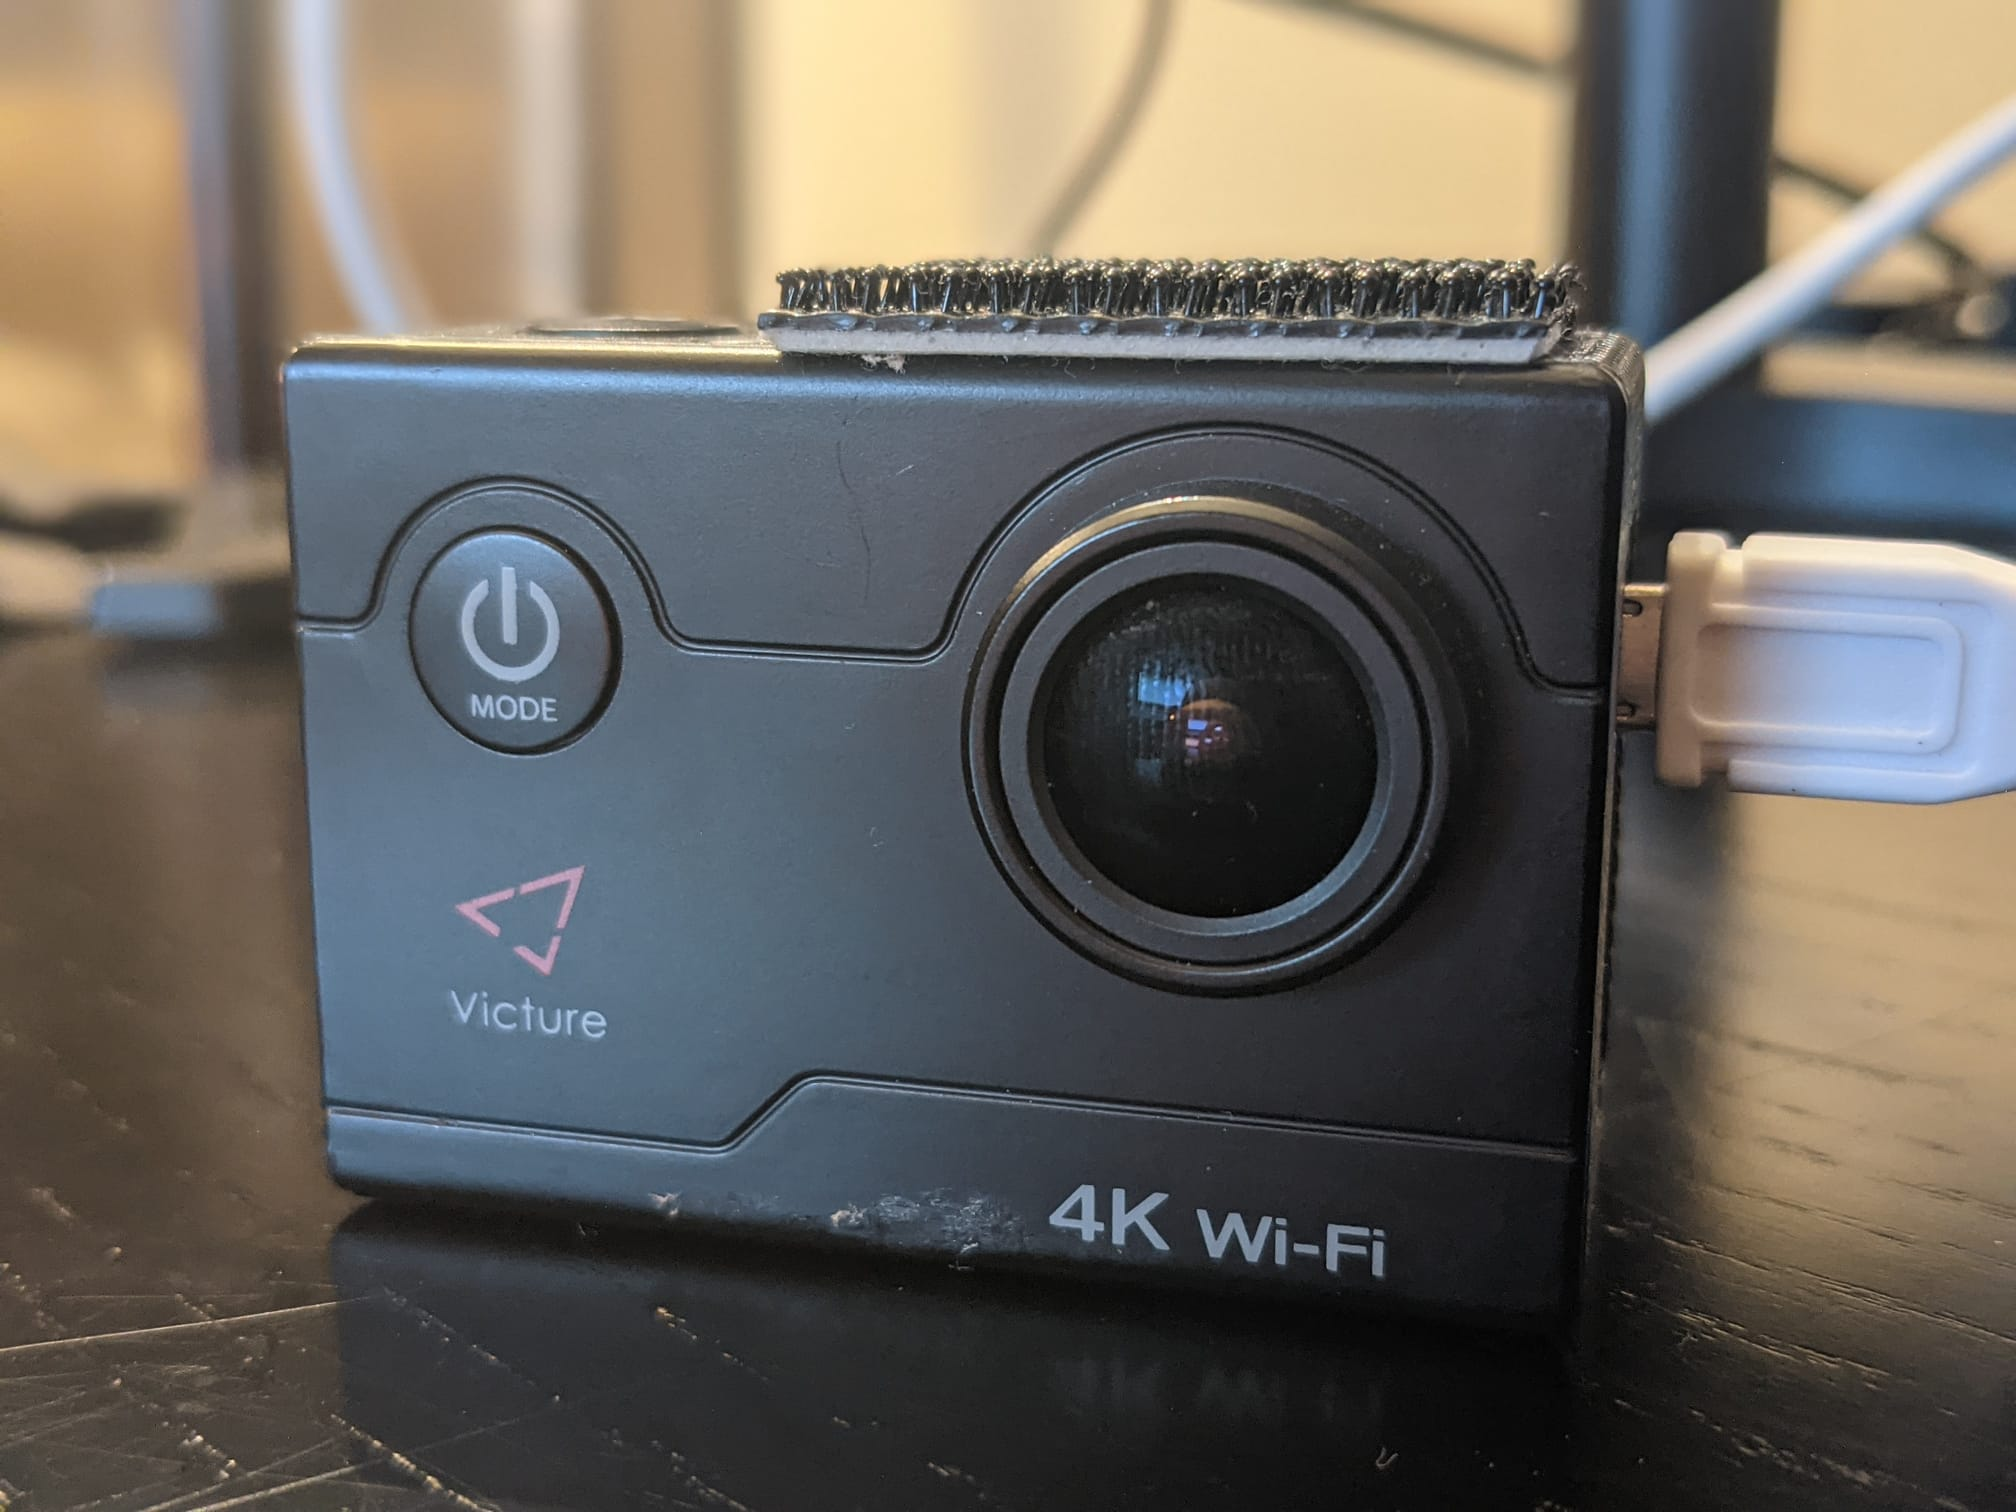
\includegraphics[width=0.4\textwidth]{03/cam.jpeg}}
\end{figure}

En concreto, el sensor seleccionado es una cámara USB Victure AC600 (Fig. \ref{fig:victure}). Además, la Tabla \ref{tab:victure} recoge las características de la cámara. Finalmente, el montaje final del sistema de la cámara junto a la aeronave se muestra en la Figura \ref{fig:px4-cam}.

\begin{figure}[!ht]
 	\ffigbox[\FBwidth] {
 	    \caption[Aeronave con cámara instalada]{Aeronave con cámara instalada.}
        \label{fig:px4-cam}
    }
 	{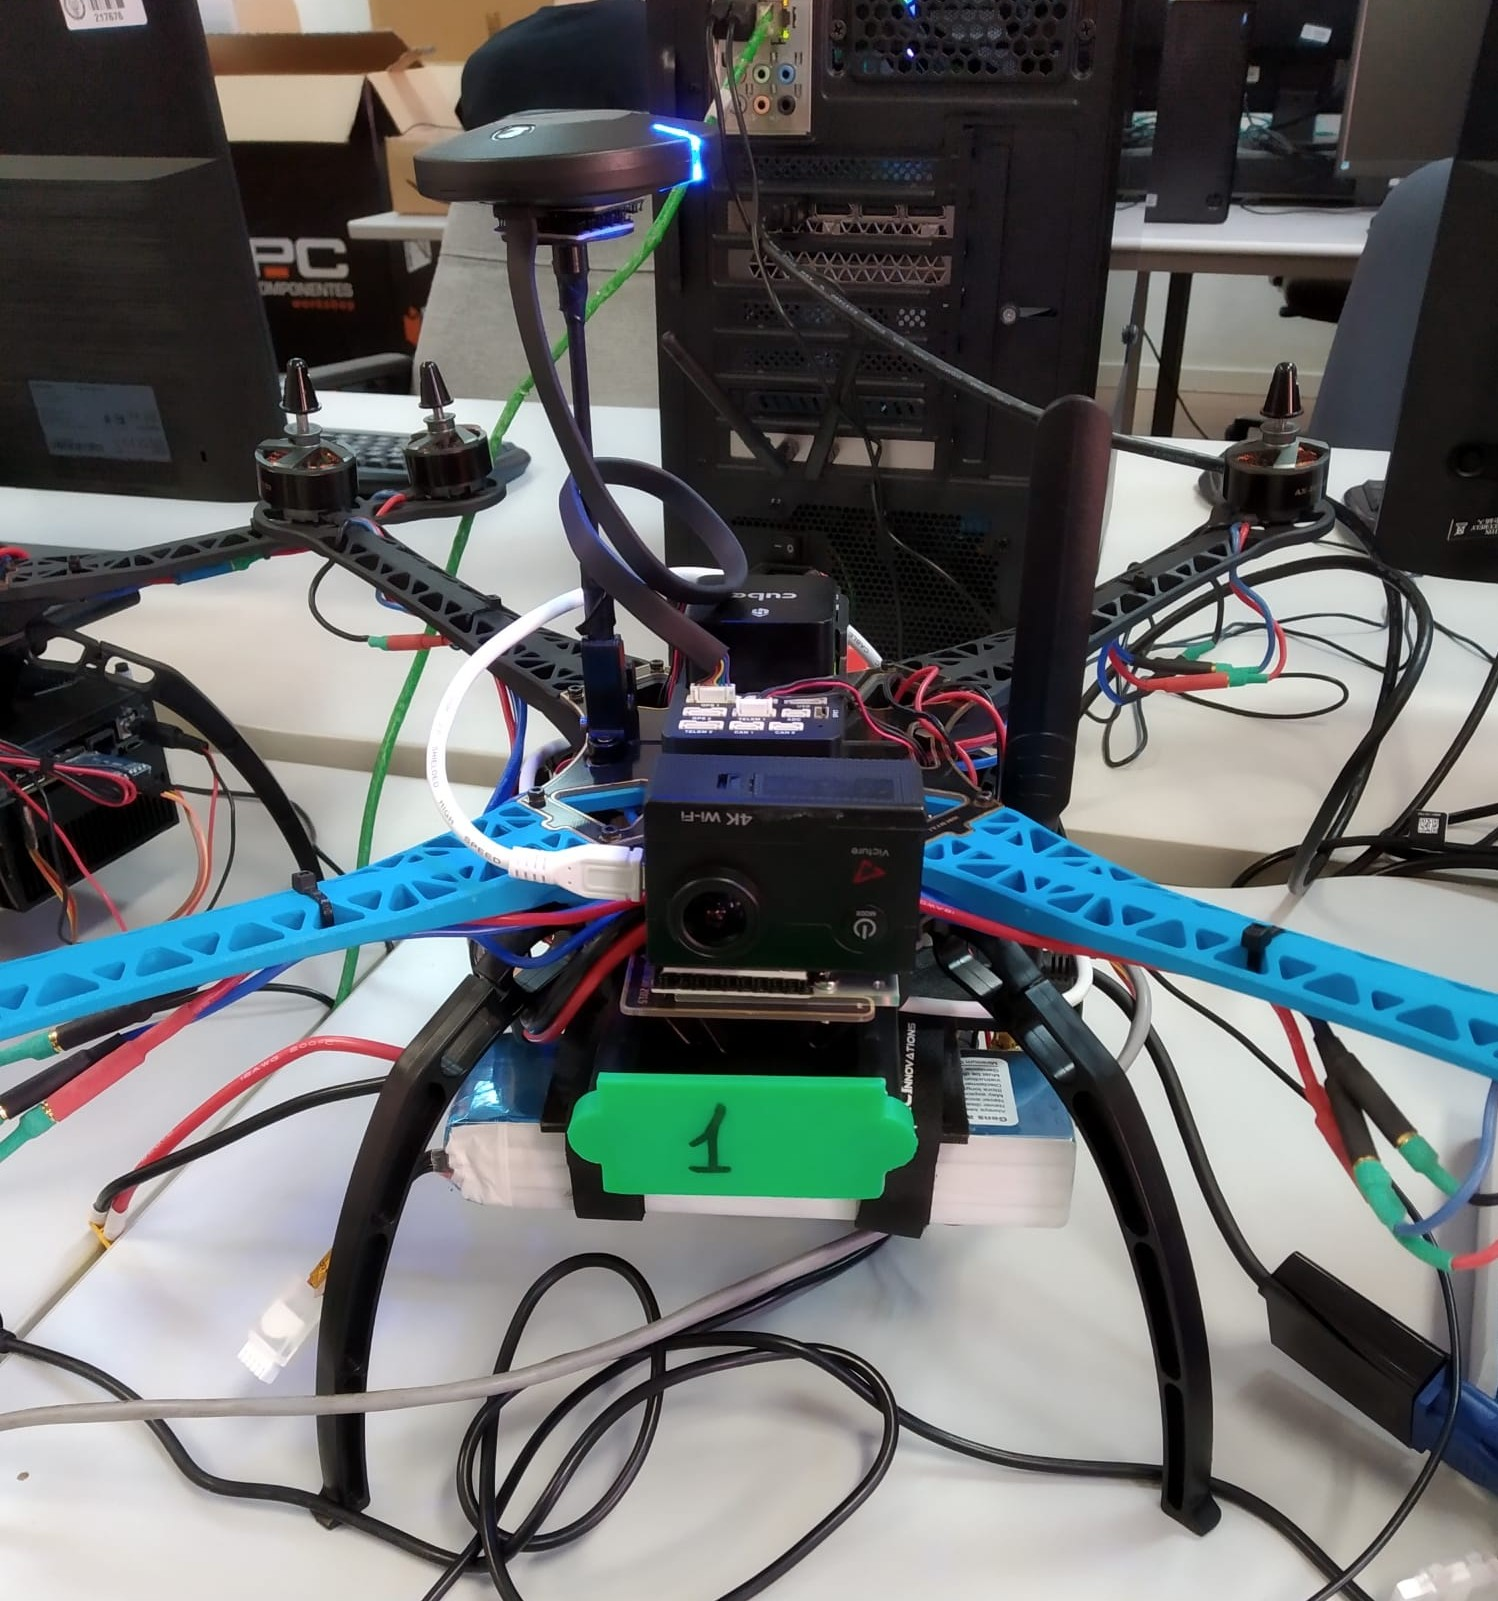
\includegraphics[width=0.62\textwidth]{03/px4-cam.jpeg}}
\end{figure}

\begin{table}[H]
	\ttabbox[\FBwidth]
	{\caption{Especificaciones de la cámara Victure AC600.} \label{tab:victure}}
	{\begin{tabular}{|c|c|}
		\hline
		\textbf{Características} & \textbf{Valores} \\
		\hline
		Peso (g)            & 78 \\
		\hline
        Tamaño (mm)         & 60x40x25 \\
        \hline
        Resolución (MP)     & 16 \\
        \hline
        FOV (º)             & 170 \\
        \hline
        Vídeo               & 4k ultraHD 25 fps \\
        \hline
		\multicolumn{2}{l}{Fuente: Victure}
	\end{tabular}}
\end{table}

\section{Software} \label{section:met-software}
El sistema operativo utilizada durante el desarrollo y las pruebas ha sido Ubuntu, la distribución de Linux basada en Debian. En concreto, la edición utilizada es la versión con soporte de largo plazo, \textit{Ubuntu 18.04.3 LTS (\emph{Bionic Beaver})} \cite{ubuntu}. El motivo de esta elección es que Ubuntu suele ser la primera opción en aplicaciones relacionadas con el software libre y la robótica. Además, como veremos en a lo largo de la sección, las principales herramientas de simulación de drones utilizan esta plataforma.

El lenguaje elegido para el desarrollo de la aplicación ha sido Python \cite{python}. Este lenguaje creado a principios de 1990 por Guido van Rossum en los Países Bajos es un lenguaje de programación interpretado, interactivo y orientado a objetos. Sus principales ventajas, que han motivado su elección para este proyecto, son una sintaxis muy clara y su portabilidad. En concreto, la versión utilizada es \textit{Python v2.7.17}. \\
Además, para ciertos aspectos del desarrollo se ha utilizado también C++ \cite{cpp}. C++ es un lenguaje de programación multiparadigma diseñado en 1979 por Bjarne Stroustrup. La intención de su creación fue extender al lenguaje de programación C mecanismos que permiten la manipulación de objetos. En concreto, la versión \textit{C++14} junto al compilador versión \textit{g++ 7.5.0}.

La plataforma robótica de software seleccionada es ROS. Además de ser la plataforma de uso más extendido, dispone de librerías en diferentes lenguajes que facilitan su uso. Una de ellas es \emph{rospy} \cite{rospy}, un cliente para Python que permite interactuar rápidamente con los nodos, servicios y parámetros de ROS. \\
ROS posee diferentes paquetes que facilitan el desarrollo de software en múltiples ámbitos. Dentro de la robótica aérea, existe una colección de nodos de comunicación extendible MAVLink para ROS conocida como \textit{MAVROS} (\emph{Micro Air Vehicles ROS}) \cite{mavros}. Este paquete de ROS proporciona un controlador de comunicación para varios autopilotos con protocolo de comunicación MAVLink, junto a una colección de nodos, servicios y parámetros que aseguran una correcta comunicación con la aeronave. La versión de MAVROS es \textit{v1.9.0} con la colección de mensajes de \textit{MAVLink v2021.3.3}.

\newpage
Para el procesamiento de imágenes, se ha elegido \textit{OpenCV} (Open Source Computer Vision) \cite{opencv}. OpenCV es una biblioteca de código abierto C++/Python/Java (escrita de forma nativa en C ++) utilizada en Visión por Computador. Entre los métodos clásicos y de última generación que incluye, se pueden encontrar varias funciones adecuadas para reconocimiento facial, seguimiento ocular, establecimiento de marcadores para realidad aumentada, etc. Debido a su excelente rendimiento, esta biblioteca ha logrado convertirse en el estándar \emph{de facto} en visión artificial para todo tipo de usuarios. La versión utilizada es \textit{v3.2.0}.

Otra biblioteca muy útil para el trabajo matricial con imágenes es \textit{NumPy} \cite{numpy}. NumPy es una biblioteca para Python que da soporte para crear vectores y matrices grandes multidimensionales, junto con una gran colección de funciones matemáticas de alto nivel para operar con ellas. La versión utilizada es la \textit{v1.13.3}.

\subsection{Simulación} \label{section:met-sim}
Entre los drones utilizados se ha introducido en la sección anterior el 3DR Iris simulado. Tal como se ha adelantado, la simulación se realiza mediante el SITL de PX4 y sobre el simulador \emph{Gazebo}. Este simulador de código abierto es por excelencia el más utilizado en aplicaciones de robótica y visión artificial. Debido a su gestión abierta permite la integración de múltiples vehículos, mundos, sensores, físicas, etc. \\
La versión utilizada durante el proyecto es \textit{Gazebo9}. El modelo del Iris simulado en el simulador se puede observar en la Figura \ref{fig:iris-sim}. El modelo lleva incluído dos \emph{plugins} que le permiten obtener imágenes (una frontal y otra ventral) de modo similar a una cámara.

\begin{figure}[!ht]
 	\ffigbox[\FBwidth] {
 	    \caption[3DR Iris simulado mediante Gazebo]{3DR Iris simulado mediante Gazebo.}
        \label{fig:iris-sim}
 	}
 	{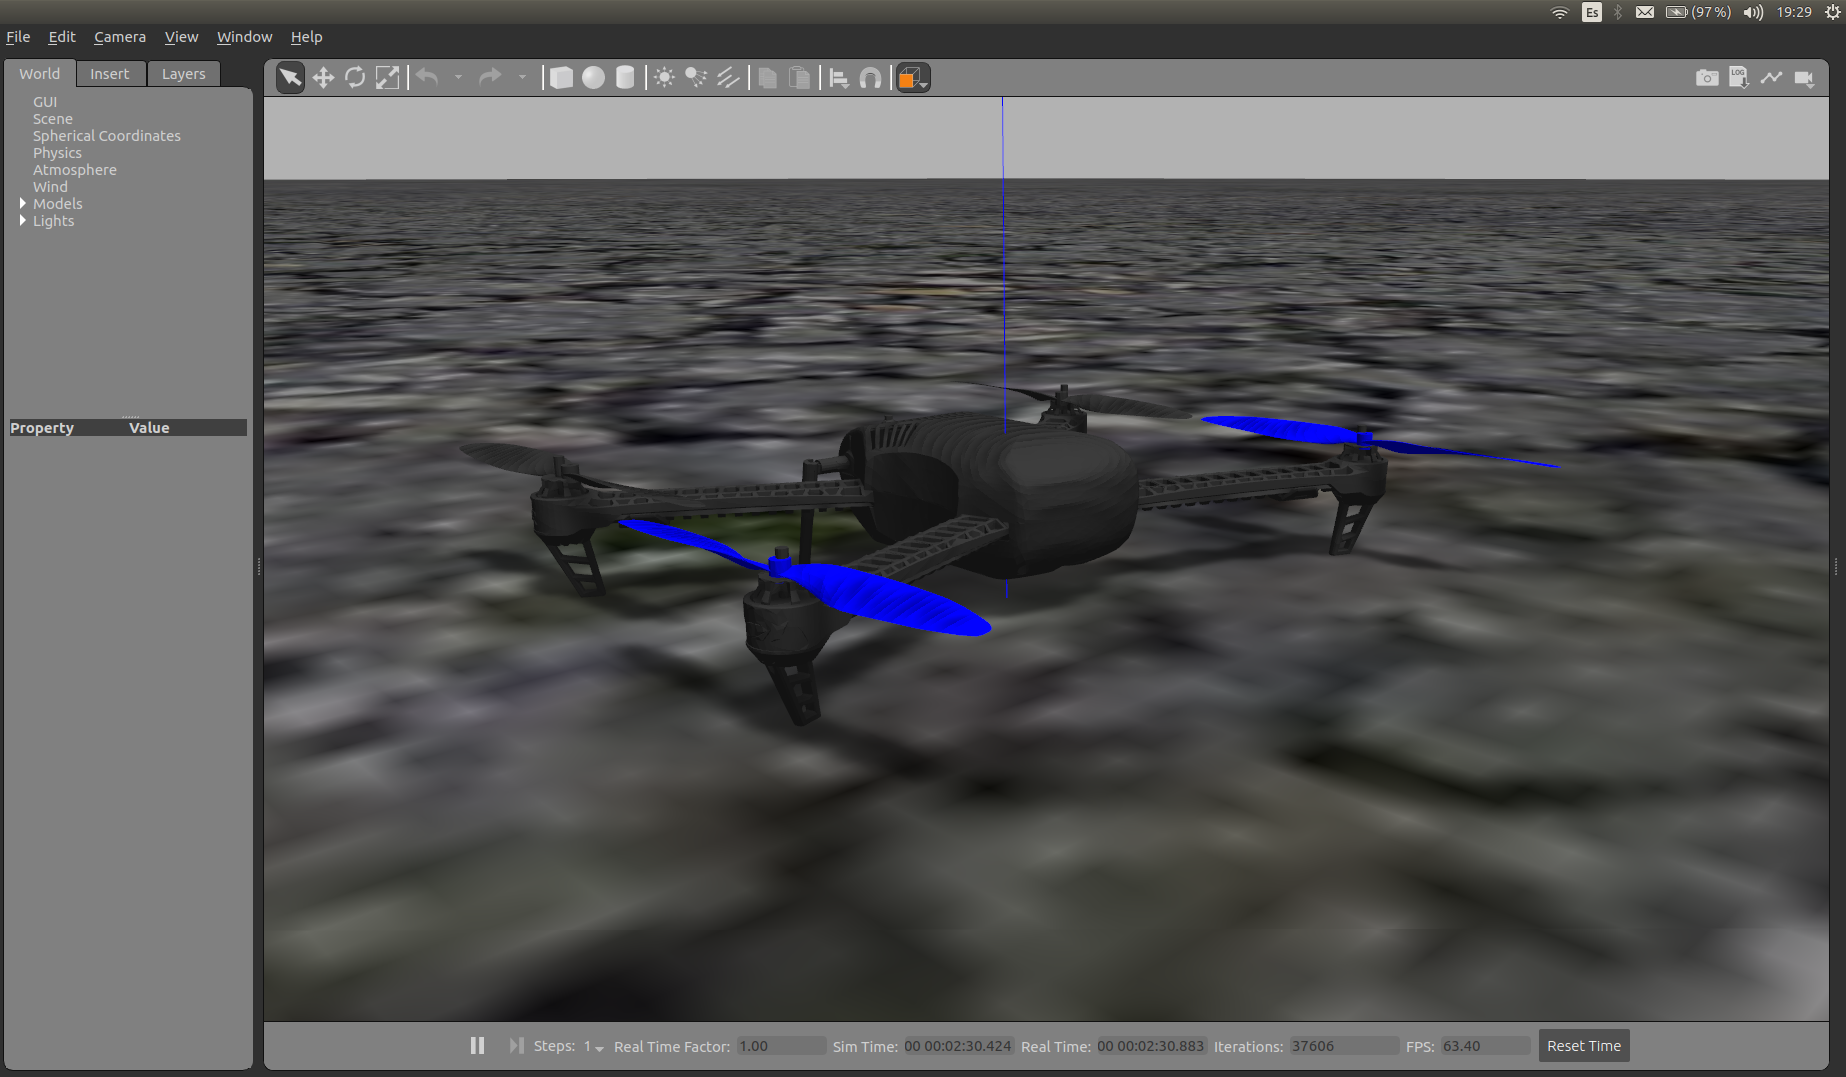
\includegraphics[width=\textwidth]{03/drone-sim.png}}
\end{figure}

\newpage
El firmware utilizado por la controladora es PX4 con la versión v1.11.3, cuyo esquema de SITL se puede observar en la Figura \ref{fig:sitl-px4}. 

\begin{figure}[!ht]
 	\ffigbox[\FBwidth] {
 	    \caption[Esquema de PX4 sobre SITL]{Esquema de PX4 sobre SITL \cite{px4}.}
        \label{fig:sitl-px4}
 	}
 	{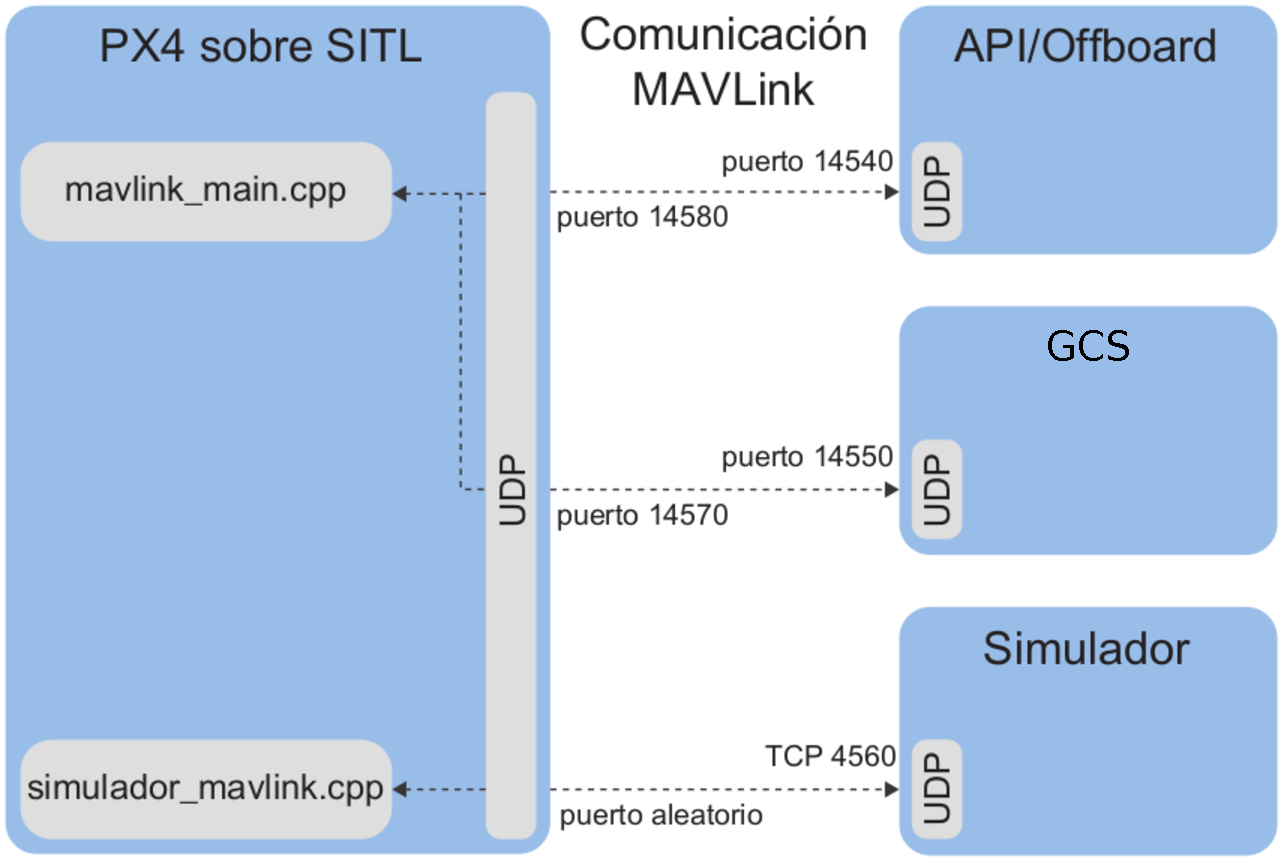
\includegraphics[width=0.9\textwidth]{03/px4-sitl.pdf}}
\end{figure}

\subsection{NVIDIA JetPack} \label{section:met-jetpack}
El dispositivo embebido utilizado, la NVIDIA Jetson AGX Xavier, sigue unas pautas de diseño integradas muy optimizadas. NVIDIA desarrolla y mantiene una versión personalizada de Ubuntu Linux, llamada NVIDIA JetPack, y está disponible para descargar e instalar como firmware de la placa \cite{jetpack}. Esta implementación personalizada incluye interfaces de bajo nivel para implementar operaciones de computación paralelas (CUDA) y varias optimizaciones SDK (kits de desarrollo de software), como TensorRT. \\
Para el sistema desarrollado, la versión utilizada es \textit{JetPack 4.6} (L4T 32.6.1).

\subsection{Aprendizaje profundo}\label{section:met-aprend}
Para este trabajo, uno de los objetivos es el desarrollo de una aplicación de aprendizaje profundo en un dron, por lo que no ha sido necesario diseñar y desarrollar una red neuronal. \\
En cambio, se ha utilizado una ya creada y ampliamente usada, YOLO (\emph{You Only Look Once}). YOLO es un sistema de detección de objetos en tiempo real de última generación, diseñado por Joseph Redmon hasta su tercera versión \cite{yolov3}. Tras el abandono del autor, fue continuada por Alexey Bochkovskiy, creador de las versiones más actuales \cite{bochkovskiy2020yolov4}. \\
Su enfoque, muy novedoso en su lanzamiento, permite alcanzar velocidad de ejecución muy elevadas. Con su método, la red neuronal se aplica una única vez sobre la imagen. Esta red divide la imagen en regiones y predice cuadros delimitadores y probabilidades para cada región.

La versión utilizada de la red para este trabajo es la \textit{YOLOv4}. Se han utilizado la configuración y pesos por defecto de la versión YOLOv4 y YOLOV4-tiny. Dichos pesos se han obtenido entrenando con la base de datos Microsoft COCO (\emph{Common Objects in COntext}) \cite{lin2014microsoft}, la cual posee 80 clases diferentes y más de 300.000 imágenes y un millón y medio de objetos etiquetados.

\section{Método} \label{section:met-met}
La metodología seguida durante el desarrollo es la filosofía del código libre. Todo el código se encuentra disponible en abierto en \emph{GitHub} \cite{github}. \emph{GitHub} es una plataforma de desarrollo colaborativo para alojar proyectos utilizando el sistema de control de versiones \emph{git}. Esta plataforma permite además una metodología en espiral con incidencias y parches.

El código fuente del proyecto se encuentra en diferentes repositorios públicos. Parte del código se aloja en \emph{JdeRobot/drones}\footnote{\url{https://github.com/JdeRobot/drones}} (rama \lstinline{melodic-devel}, versión 1.3.10), mientras que otra parte del código se puede encontrar en \emph{RoboticsLabURJC/2021-tfm-pedro-arias}\footnote{\url{https://github.com/RoboticsLabURJC/2021-tfm-pedro-arias}}. \\
El software en el repositorio \emph{drones} ha sido desarrollado por la asociación de robótica \emph{JdeRobot} \cite{jderobot}, ligada a la Universidad Rey Juan Carlos (URJC), y entre sus desarrolladores se encuentra el autor de este trabajo. El código del segundo repositorio ha sido desarrollado en su totalidad por el autor y con motivo de este proyecto.

Además, a lo largo del proyecto se han mantenido reuniones semanales (o cada dos semanas, en función del periodo del año) con los tutores mediante videoconferencia. Para cada una de estas reuniones, se ha desarrollado una presentación con los progresos y avances realizados durante cada periodo de tiempo. Dichas reuniones ha permitido mantener un flujo de información constante entre alumno y tutores, recibir periódicamente realimentación del trabajo realizado y fijar los objetivos a corto plazo para el siguiente periodo de trabajo.

\end{document}